\chapter{Introdução}\label{cap:introducao}

Muitos dos problemas encontrados no dia-a-dia podem possuir inúmeras soluções, que em geral detêm um fator de satisfação associado (e.g.: lucro obtido, custo de utilização).
Nessa linha, o ramo da otimização atua no estudo destes de modo a buscar minimizar ou maximizar o valor da função objetivo (satisfação) associada.

Conforme pode ser visto na Figura~\ref{fig:espacoDeBusca}, um método de otimização explora o espaço de busca a procura da solução que apresente o melhor valor de função objetivo.

\begin{figure}[htpb]
    \centering
    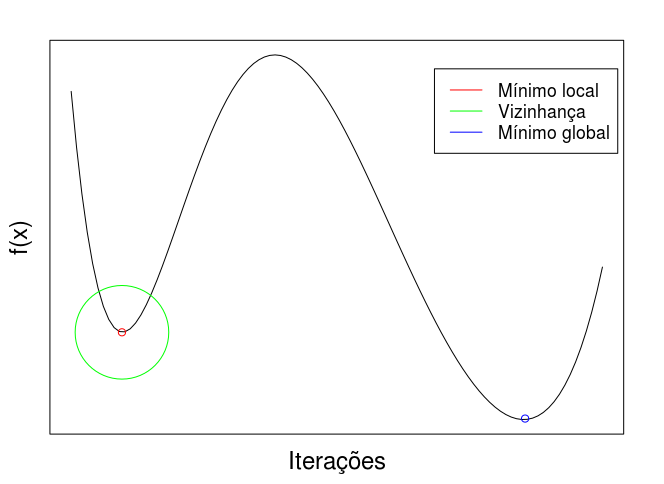
\includegraphics[scale=0.6]{figuras/desenharCurva-semEixo.png}
    \caption{Espaço de busca explorado por um método de otimização. São indicados mínimo local, mínimo global e vizinhança, conceitos que serão definidos a frente.}
    \label{fig:espacoDeBusca}
\end{figure}

Quando é necessário resolver problemas de otimização, um campo promissor é o das meta-heurísticas, contudo estes algoritmos podem demandar muito tempo de processamento, especialmente ao se resolver problemas com grandes instâncias. Isto posto, podemos ressaltar a importância de utilizar métodos eficientes para resolução de tais problemas.

Uma parte importante no universo das meta-heurísticas são os algoritmos de busca que, inicialmente, recebem uma solução para um problema e rastreiam seu espaço de busca para então retornar a melhor solução encontrada.
O espaço de busca é um super conjunto de algumas estratégias de vizinhança para a solução atual e as que surgirem.

Uma boa alternativa para melhorar o tempo de processamento destes problemas é pela utilização de programação paralela~\cite{handbookmeta}.
A maioria dos algoritmos de otimização até então projetados foram feitos para funcionarem de forma ``naturalmente'' sequencial, criando uma árdua tarefa, muitas vezes hercúlea, para os programadores que desejam alterar a implementação do algoritmo para rodar de forma paralela.
A abordagem mais utilizada para paralelização de meta-heurísticas consiste em escolher métodos ou partes do método que podem ser executadas independentemente e lançar sua execução paralela (\emph{Bag-of-Tasks}).
Não obstante apenas alguns trabalhos científicos são dedicados a realmente re-projetar estes algoritmos para aproveitar o poder de arquiteturas paralelas de forma profunda~\cite{vns2015, jpdc2017, endm2018:araujo}.

% Sugestão [MARZULO]
Em abordagens tradicionais para paralelização de aplicações são empregadas arquiteturas \emph{Multiple Instruction Multiple Data} (\emph{MIMD})~\cite{flynn1972}, onde cada elemento de processamento possui \emph{streams} de instruções e dados independentes.
Desta forma, o desenvolvedor pode particionar as tarefas de sua aplicação para que sejam executadas em \emph{threads} ou processos, mapeadas nos elementos de processamento.
A comunicação entre tarefas pode ser realizada por memória compartilhada (multiprocessadores ou \emph{multicores}) ou por troca de mensagens (como em \emph{clusters} de computadores).
% A abordagem mais direta de paralelizar uma aplicação é usando múltiplas threads ou processos numa máquina com múltiplos processadores (ou múltiplos cores) ou utilizando muitos computadores (e.g., um cluster de máquinas), i.e. usando uma arquitetura Multiple Instruction Multiple Data (MIMD)~\cite{flynn1972}.
Estes processadores seguem o modelo de Von Neumann, no qual a execução de uma instrução é guiada pelo fluxo de controle, de forma que a ordem das instruções no programa prescreve o que o processador deve fazer passo a passo.
Este modelo assume que um \textit{program counter} é usado para indicar a próxima instrução a ser executada e estas podem alterar o estado da máquina ao alterar valores de uma estrutura de armazenamento global, como um banco de registradores, cache ou memória principal.

Trabalhos recentes em modelos e linguagens de programação paralela~\cite{trebuchetijhpsa,1473,1136512,Gupta:2011:DES:2155620.2155628,tbbflow,journals/pc/BosilcaBDHLD12,Giorgi2014} geraram novos \emph{frameworks} para o modelo de programação dataflow, em diferentes níveis de abstração e granularidade, como solução para representar programas considerando as operações como ponto de vista principal, permitindo assim uma modelagem mais fácil de muitos problemas ao alta performance.
Está claro que em alguns casos o esforço de programação (medido em termos de tempo de programação ou linhas de código) é consideravelmente reduzido quando se utiliza programação dataflow para paralelizar as aplicações, se compararmos com as ferramentas tradicionais como OpenMP ou Pthreads.
Além disso, o desempenho da execução do aplicações desenvolvidas conforme o modelo dataflow pode ser comparado com métodos tradicionais \cite{trebuchetijhpsa,lcswamca}.
% Teve um revisor que contestou esse "de fato", mantenho isso? 
% Corroborando assim dataflow como uma técnica \textit{de facto} para programação paralela, de forma que oferece facilidade de programação e boa performance.

A Figura~\ref{fig:dataflowExemplo} mostra um paralelo entre a versão Von Neumann, no quadro A e a implementação do mesmo código no modelo dataflow, exemplificada no quadro B.
Pelo quadro B pode-se perceber que a execução das operações $x + y$ e $k * j$ podem ser executadas em qualquer ordem, ou mesmo simultaneamente, sem alterar o resultado final da execução.

\begin{figure}[htpb]
    \centering
    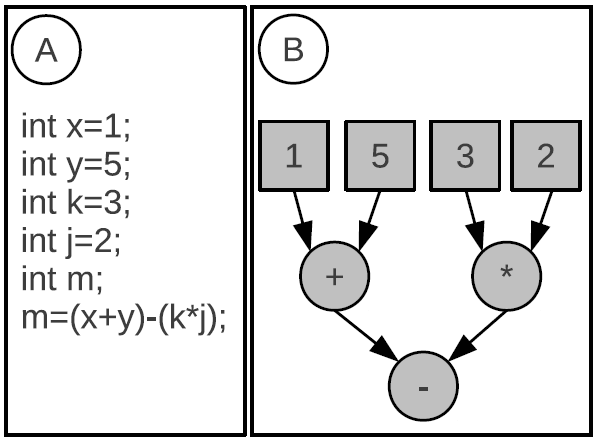
\includegraphics[scale=0.6]{figuras/dataflow/dataflowExemplo.png}
    \caption{Exemplo de conversão código para grafo de dependências, conforme apresentado em~\cite{teseMarzulo}.
    O quadro A mostra um trecho de código e o quadro B o grafo dataflow associado.}
    \label{fig:dataflowExemplo}
\end{figure}

Usualmente a programação dataflow é feita instanciando trechos de código e os conectando em um grafo de acordo com suas dependências de dados, livrando assim o programador de grande parte da complexidade da programação paralela uma vez que esta, bem como a sincronização, são realizados pelo ambiente de execução dataflow.
O modelo dataflow expõe naturalmente o paralelismo, instruções são executadas conforme suas dependências de dados (na ordem do fluxo de dados, dataflow), i.e., instruções são disparadas assim que seus operandos estão disponíveis, dessa forma o desafio passa a ser modelar o grafo de dependências das operações tendo como uma importante decisão a se tomar o tamanho do grão de cada nó do grafo de forma a comportar o paralelismo sem sobrecarregar o algoritmo podendo assim causar um \emph{overhead} desnecessário na troca de mensagens.

Problemas NP-Difíceis~\cite{GareyJohnson1990} surgem de cenários práticos, como o roteamento de um conjunto de veículos para entregas e coletas, ou visitar um conjunto de cidades percorrendo a menor rota possível.
Este último sendo conhecido como Problema do Caixeiro Viajante (PCV), um dos mais importantes (e não resolvidos) problemas no campo da ciência da computação.
Devido a sua combinatoriedade natural, não existe algoritmo conhecido que resolva o PCV em tempo polinomial.
Todavia, muitos algoritmos heurísticos e combinações de métodos exatos com métodos heurísticos são capazes de resolver o PCV para instâncias com milhares de cidades.
Como uma variante menos explorada do PCV, consideramos o Problema da Mínima Latência (PML), que é uma variante do PCV onde todos os nós precisam ser visitados, mas o custo é o somatório do acumulado das distâncias ponto a ponto.

Muitos trabalhos recentes produziram algoritmos que obtiveram resultados eficientes utilizando RVND~\cite{souza2010, silva2012,subramanian2013}, cuja ideia principal é que ao se atingir um mínimo local para uma estratégia de vizinhança ainda pode existir um vizinho em outra vizinhança com valor de função objetivo melhor que o já encontrado, o que motivou a implementação de uma versão distribuída.
O DVND, proposto em~\cite{RIOS201839}, é uma versão paralela do método de busca VND, adotando-se uma visão dataflow para o algoritmo é possível uma implementação conforme a encontrada em \cite{df-dvnd2018}.
A arquitetura multi-core do DVND torna possível explorar diferentes vizinhanças simultaneamente (com diferentes implementações de busca local), e escolher o melhor resultado dos métodos de busca.
Não obstante, os autores que obtiveram o estado da arte nos resultados para o PML não chegaram a estender a implementação do DVND para múltiplos e independentes nós de processamento devido a problemas de performance, serialização de dados e controle de fluxo utilizando a tecnologia MPI~\cite{jpdc2017}.
Por esse motivo esse trabalho propõe uma nova implementação do DVND capaz de lidar com múltiplos nodos de maneira mais natural, modelando o método como um grafo dataflow e usando o framework em Python para dataflow Sucuri~\cite{sucuri-original}.

% Comentei isso porque achei que ficou meio descontextualizado
%Entretanto, no mundo real, os problemas tendem a ser inter relacionados uns aos outros e resolver separadamente as subpartes do problema não necessariamente resolve o problema em si. Este é o caso em vários aplicações práticas de problemas clássicos como o Problema da Mochila ~\cite{Pisinger:1995} e o Problema do Caixeiro Viajante~\cite{Dantzig:1954}. Muitas outras variantes desses problemas clássicos podem ser encontradas na literatura, contudo poucos são bem sucedidos ao combinar os problemas de forma a desaviar os algoritmos no estado da arte atual.

%In this paper we deal with the Traveling Thief Problem (TTP) \cite{Bonyadi:2013}, a combination of the Traveling Salesman Problem (TSP) and the 0/1 Knapsack Problem (KP), using both classic well known optimization problems.
% Preciso citar isso?
%These two components have been merged in such a way that the optimal solutions for each problem do not necessarily correspond to an optimal TTP solution~\cite{wagner:2017}.
%A practical application for the TTP is indicated by Mei et al.~\cite{mei:2015} and consists of a routing problem with service profit, where each costumer has a demand and a service profit, and the travel cost depends on the load of the vehicle.
%Another evidence for the importance of considering the impact of vehicle load in travel costs is related to carbon emissions and can be seen in the Green Vehicle Routing Problem literature~\cite{Lin:2014}.
%By studying the TTP it is possible to perform a systematic investigation of interactions between two hard optimization problems, to eventually help solving real-word problems more efficiently~\cite{Bonyadi:2016}.

\section{Motivação}\label{sec:motivacao}

Inúmeras aplicações práticas podem utilizar meta-heurísticas para resolver problemas de otimização, sendo comum para muitos desses processos sua etapa final ser constituída de um algoritmo de busca local.
Este por sua vez faz uso de estratégias de vizinhança para enumerar o espaço de busca.
% (e.g. Swap, 2-Opt, OrOpt-2, ..., etc)
Versões clássicas do processos de busca local utilizam uma vizinhança em conjunto com uma estratégia de exploração (Primeira melhora, Melhor vizinho).

% Cito o VND ao mencioná-lo aqui?
Poucos são os trabalhos da literatura que combinam estratégias de vizinhança diferentes como em \emph{Variable Neighborhood Descent} (\emph{VND}) e mais raros são os trabalhos que usam diferentes estratégias de exploração de vizinhança como em \cite{vns2015}.

\section{Objetivos} \label{sec:objetivos}

% Emprego de múltiplas estratégias de vizinhança com uso de GPU para solução de problemas de otimização
Este estudo visa propor estratégias diferenciadas de solução de problemas de otimização, para tanto podemos enumerar os seguintes objetivos:
\begin{itemize}
    \item{A investigação do uso de estratégias distintas de vizinhanças almeja a realização de uma busca mais extensa no espaço de soluções, contudo isto aumenta sua complexidade computacional, o que abre caminho para o item seguinte;}
    \item{Propor algoritmos paralelos que se beneficiam de tecnologias emergentes, porém ainda pouco exploradas no ramo da pesquisa operacional, que é a utilização de aceleração pelo uso de placas gráficas;}
    \item{Utilizar melhor os recursos usados no processamento realizado ao aproveitar computações realizadas em nós diferentes.}
\end{itemize}

O objetivo final é propor um método que seja capaz de fazer uso de múltiplas estratégias de vizinhança aproveitando recursos de paralelização de grão fino e grão grosso sem precisar acoplar a solução a um problema específico.

\section{Estrutura deste documento}\label{sec:estrutura}

O restante deste trabalho é organizado conforme o segue:

\begin{itemize}
    \item Capítulo~\ref{cap:conceitos}: descreve os fundamentos teóricos e termos utilizados nessa dissertação, no desenvolvimento deste capítulo são caracterizados e ilustrados os termos e meta-heurísticas utilizados por descrições independentes;
    \item Capítulo~\ref{cap:metodologia}: descreve e apresenta os algoritmos propostos para resolver o Problema da Mínima Latência mas não se limitando a este problema. Este capítulo detalha os métodos bem como seus componentes e pseudocódigos;
    \item Capítulo~\ref{cap:resultados}: mostra os resultados computacionais deste trabalho. Os métodos Dataflow DVND e GDVND propostos podem utilizar diferentes estratégias e da mesma forma podem ser aplicados a problemas variados;
    \item Capítulo~\ref{cap:conclusao}: apresenta as conclusões do trabalho desenvolvido nessa dissertação com as propostas de trabalhos futuros.
\end{itemize}
